\documentclass[a4paper,12pt]{report}

\usepackage{cmap}
\usepackage[T2A]{fontenc}
\usepackage[utf8]{inputenc}
\usepackage[english,russian]{babel}
\usepackage{listings}
\usepackage{amsmath}
\usepackage{amsfonts}
\usepackage{float}
\usepackage{csquotes}
\usepackage{hyphenat}

% \usepackage{titlesec}
% \newcommand{\sectionbreak}{\clearpage}

\usepackage{graphicx}
\graphicspath{ {./images/} }

\usepackage{xcolor}
% \usepackage{courier}

\definecolor{buzzlightyear}{HTML}{8757A5}
\definecolor{grass}{HTML}{738D06}
\definecolor{sand}{HTML}{F18A2B}
\definecolor{comment}{HTML}{8E908B}

\lstdefinestyle{habrstyle}{
    backgroundcolor=\color{white},   
    commentstyle=\color{comment},
    keywordstyle=\bfseries\color{buzzlightyear},
    numberstyle=\tiny\color{comment},
    stringstyle=\color{grass},
    basicstyle=\ttfamily\footnotesize,
    breakatwhitespace=false,         
    breaklines=true,                 
    captionpos=b,                    
    keepspaces=true,                 
    numbers=left,                    
    numbersep=5pt,                  
    showspaces=false,                
    showstringspaces=false,
    showtabs=false,                  
    tabsize=4
}

\lstset{style=habrstyle}

\author{Луняк Николай}
\title{Лабораторная работа 3}
\date{\today}

\begin{document}
    \maketitle
    \tableofcontents
    \listoffigures
    \lstlistoflistings
    
    \chapter{Пробуем примеры из \texttt{chap03.ipynb}}
    
    Тут надо просто посмотреть на примеры из третьей главы, послушать всякие звуки и убедиться, что все работает.
    
    \begin{figure}[H]
        \centering
        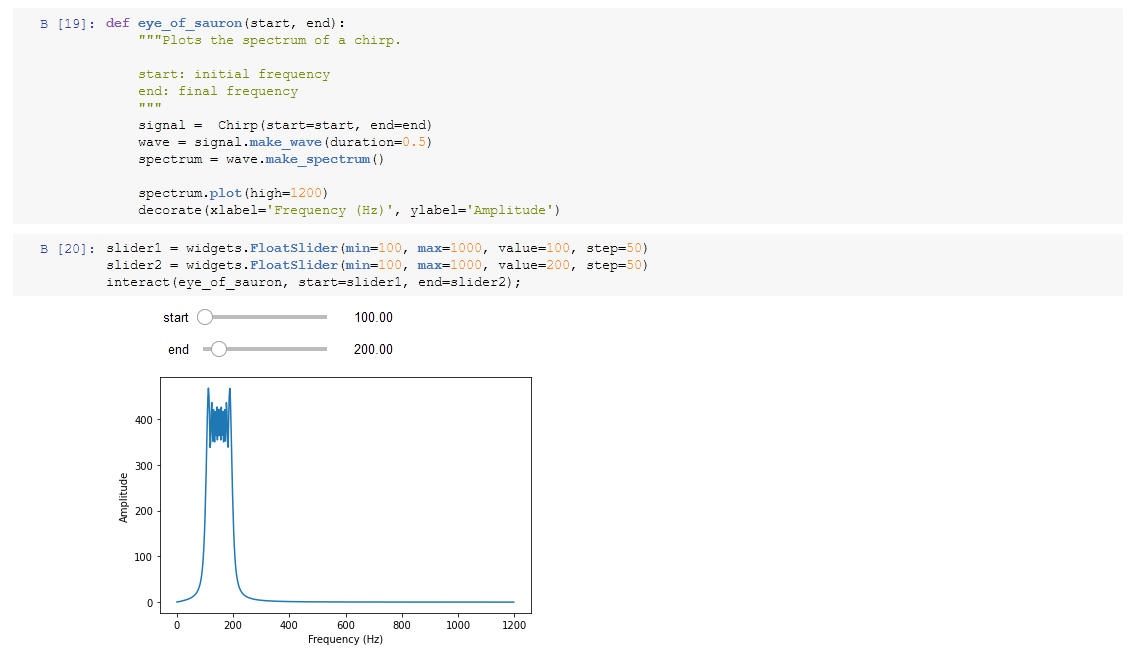
\includegraphics[width=\textwidth]{ex1_it_works.png}
        \caption{Работает}
        \label{fig:ex1_it_works}
    \end{figure}
    
    Проверять разные окна будем вот так.
    
\begin{lstlisting}[language=Python,caption=Проверка окон]
wave = signal.make_wave(duration)
wave.window(np.bartlett(len(wave)))
spectrum = wave.make_spectrum()
spectrum.plot(high=880)
decorate(xlabel='Frequency (Hz)')

wave = signal.make_wave(duration)
wave.window(np.blackman(len(wave)))
spectrum = wave.make_spectrum()
spectrum.plot(high=880, color='red')
decorate(xlabel='Frequency (Hz)')

wave = signal.make_wave(duration)
wave.window(np.hanning(len(wave)))
spectrum = wave.make_spectrum()
spectrum.plot(high=880, color='green')
decorate(xlabel='Frequency (Hz)')

wave = signal.make_wave(duration)
wave.window(np.kaiser(len(wave), 10))
spectrum = wave.make_spectrum()
spectrum.plot(high=880, color='orange')
decorate(xlabel='Frequency (Hz)')
\end{lstlisting}

    \begin{figure}[H]
        \centering
        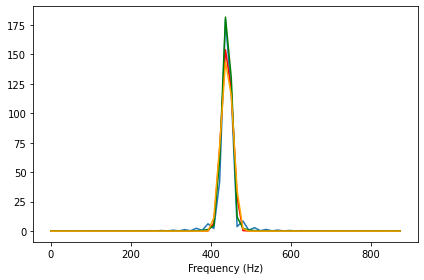
\includegraphics[width=0.75\textwidth]{ex1_testing.png}
        \caption{Все вместе}
        \label{fig:ex1_testing}
    \end{figure}
    
    \chapter{Делаем \texttt{SawtoothChirp}}
    
    \section{Основной код}
    
    В задании просят за основу взять \texttt{Chirp}.
    
\begin{lstlisting}[language=Python,caption=Реализация своего пилообразного \texttt{Chirp}'а]
class MySawtoothChirp(Chirp):
    def evaluate(self, ts):
        freqs = np.linspace(self.start, self.end, len(ts) - 1)
        
        dts = np.diff(ts)
        dphis = PI2 * freqs * dts
        
        phases = np.cumsum(dphis)
        phases = np.insert(phases, 0, 0)
        
        cycles = phases / PI2
        frac, _ = np.modf(cycles)

        ys = self.amp * frac
        return ys
\end{lstlisting}

    Деление на \texttt{PI2} я сделал по сути \textquote{для красоты}, чтобы период был как бы $2\pi$.

    \section{Проверка}

    Проверим сегменты в секундном \texttt{Wave}'е (начало и конец).

\begin{lstlisting}[language=Python,caption=Начало]
test_saw = MySawtoothChirp(start=220, end=440)
test_wave = test_saw.make_wave(duration=1, framerate=11025)
test_wave.segment(start=0, duration=0.02).plot() 
decorate(xlabel='Time (s)')
\end{lstlisting}

    \begin{figure}[H]
        \centering
        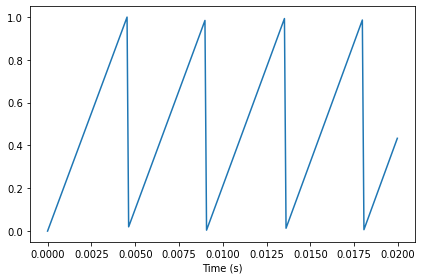
\includegraphics[width=0.75\textwidth]{ex2_start.png}
        \caption{Начало}
        \label{fig:ex2_start}
    \end{figure}

\begin{lstlisting}[language=Python,caption=Конец]
test_wave.segment(start=1-0.02, duration=0.02).plot()
decorate(xlabel='Time (s)')
\end{lstlisting}

    \begin{figure}[H]
        \centering
        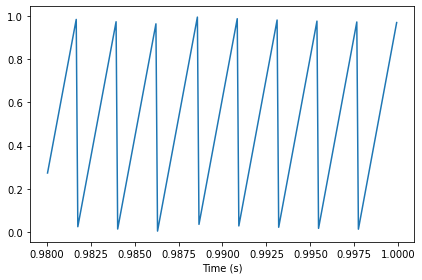
\includegraphics[width=0.75\textwidth]{ex2_end.png}
        \caption{Конец}
        \label{fig:ex2_end}
    \end{figure}
    
    \chapter{Строим специфический \texttt{SawtoothChirp}}
    
    Сделаем ровно так, как нас просят в задании.
    
\begin{lstlisting}[language=Python,caption=Создаем сигнал и ...]
signal = MySawtoothChirp(start=2500, end=3000)
wave = signal.make_wave(duration=1, framerate=20_000)
\end{lstlisting}

    Предлагаю сразу кое-что проверить.
    
\begin{lstlisting}[language=Python,caption=Проверяем его]
wave.segment(start=0.9, duration=0.02).plot()
decorate(xlabel='Time')
\end{lstlisting}

    \begin{figure}[H]
        \centering
        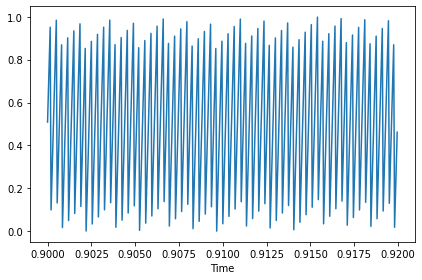
\includegraphics[width=0.75\textwidth]{ex3_initial_test.png}
        \caption{Конец интервала}
        \label{fig:ex3_initial_test}
    \end{figure}
    
    Кажется, будто бы наш сигнал начинает \textquote{скакать} вверх и вниз. Это можно исправить, увеличив \texttt{framerate}, но оставим пока так.
    
    Посмотрим, на спектр.
    
\begin{lstlisting}[language=Python,caption=Спектр]
spectrum = wave.make_spectrum()
spectrum.plot()
decorate(xlabel='Frequency')
\end{lstlisting}

    \begin{figure}[H]
        \centering
        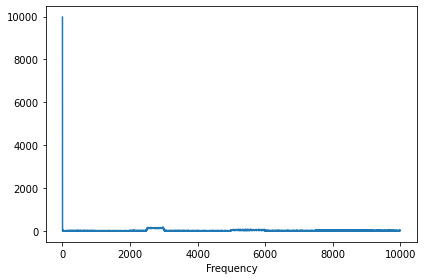
\includegraphics[width=0.75\textwidth]{ex3_first.png}
        \caption{Спектр}
        \label{fig:ex3_first}
    \end{figure}
    
    И уберем частоту в самом начале, чтобы лучше видеть форму.
    
\begin{lstlisting}[language=Python,caption=Еще спектр]
spectrum = wave.make_spectrum()
spectrum.high_pass(10)
spectrum.plot()
decorate(xlabel='Frequency')
\end{lstlisting}

    \begin{figure}[H]
        \centering
        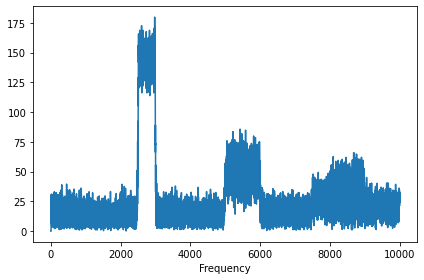
\includegraphics[width=0.75\textwidth]{ex3_second.png}
        \caption{Еще спектр}
        \label{fig:ex3_second}
    \end{figure}
    
    Похоже, тут есть некоторая уменбшающаяся величина, но при этом все как будто слишком \textquote{зашумленно}. Вот, что получается с \texttt{framerate}, увеличенным в 16 раз.
    
\begin{lstlisting}[language=Python,caption=Новый сигнал]
signal16 = MySawtoothChirp(start=2500, end=3000)
wave16 = signal.make_wave(duration=1, framerate=20_000*16)
wave16.segment(start=0.9, duration=0.02).plot()
decorate(xlabel='Time')
\end{lstlisting}

    \begin{figure}[H]
        \centering
        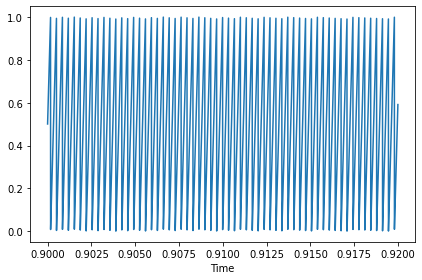
\includegraphics[width=0.75\textwidth]{ex3_signal16.png}
        \caption{Еще спектр}
        \label{fig:ex3_signal16}
    \end{figure}
    
\begin{lstlisting}[language=Python,caption=Новый спектр]
spectrum16 = wave16.make_spectrum()
spectrum16.high_pass(10)
spectrum16.plot()
decorate(xlabel='Frequency')
\end{lstlisting}

    \begin{figure}[H]
        \centering
        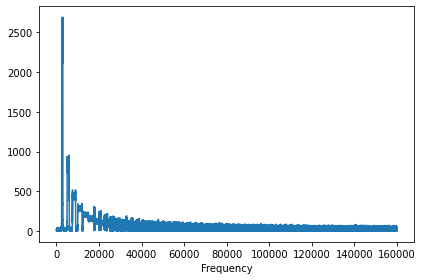
\includegraphics[width=0.75\textwidth]{ex3_spectrum16.png}
        \caption{Еще спектр}
        \label{fig:ex3_spectrum16}
    \end{figure}
    
    Теперь уже можно примерно видеть, к какой кривой стремится график.
    
    \chapter{Glissando}
    
    Начало возьму из \textquote{Rhapsody in Blue} (George Gershwin), как это советуют в ThinkDSP.
    
\begin{lstlisting}[language=Python,caption=Загрузка]
from thinkdsp import read_wave
wave = read_wave('Sounds/rhapblue11924.wav')
segment = wave.segment(start=1.35, duration=1.8-1.35)
segment.plot()
\end{lstlisting}

    \begin{figure}[H]
        \centering
        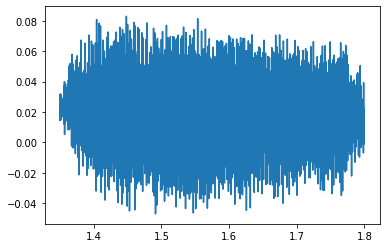
\includegraphics[width=0.75\textwidth]{ex4_wave.png}
        \caption{Визуалиация}
        \label{fig:ex4_wave}
    \end{figure}
    
\begin{lstlisting}[language=Python,caption=Спектр]
spectrum = segment.make_spectrum()
spectrum.plot()
\end{lstlisting}

    \begin{figure}[H]
        \centering
        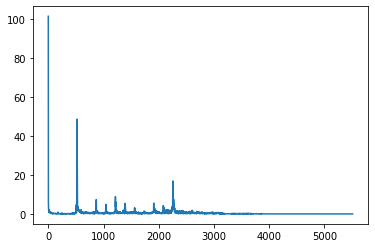
\includegraphics[width=0.75\textwidth]{ex4_spectrum.png}
        \caption{Спектр}
        \label{fig:ex4_spectrum}
    \end{figure}
    
    \chapter{Делаем \texttt{TromboneGliss}}
    
    \section{Рассуждения}
    
    Если $X$ - некоторая частота (нота), а $l_X$ - величина, означающася, насколько выдвинута кулиса, то по условию:
    
    \begin{align*}
        X &\sim \frac{1}{l_X} \\
        X &= k\cdot\frac{1}{l_X}
    \end{align*}
    
    Тогда $C_3$ (262Hz) и $F_3$ (349Hz) соответствуют некие $l_{C_3}$ и $l_{F_3}$ (причем, $l_{C_3} > l_{F_3}$).
    
    Так как:
    
    \begin{align*}
        \begin{cases}
            C_3 = k \cdot \dfrac{1}{l_{C_3}} \\
            F_3 = k \cdot \dfrac{1}{l_{F_3}}
        \end{cases}
        \Rightarrow
        F_3\cdot l_{F_3} = C_3\cdot l_{C_3}
        \Rightarrow
        X = \frac{F_3\cdot l_{F_3}}{l_X}
    \end{align*}
    
    Или:
    
    \begin{align*}
        X &= \frac{F_3\cdot l_{F_3}}{l_{F_3} + \delta l} \\
          &= \frac{F_3\cdot l_{F_3}}{l_{F_3} + t(l_{C_3} - l_{F_3})} \\
          &= \frac{F_3}{1 + t\left(\frac{l_{C_3} - l_{F_3}}{l_{F_3}}\right)} \\
          &= \frac{F_3}{1 + t\left(\frac{l_{C_3}}{l_{F_3}} - 1\right)} \\
          &= \frac{F_3}{1 + t\left(\frac{F_3}{C_3} - 1\right)} \\
    \end{align*}
    
    Где $t \in [0,1]$ - некоторая величина, принимающая значение 0 на концах периода, а 1 - в его середине и меняющаяся линейно.
    
    Если $l_X$ меняется линейно, то $X$ будет меняться обратно пропорционально квадрату $l_X$:
    
    \begin{align*}
        \frac{d X}{d l_X} = -\frac{k}{l_X^2}
    \end{align*}
    
    \section{Реализация}
    
\begin{lstlisting}[language=Python,caption=Код \texttt{MyTromboneChirp}]
class MyTromboneGliss(Chirp):
    def _get_frequency(self, ts):
        S, E = self.start, self.end
        
        # ts are normalized to [0,1]
        return E / (1 + ts * (E/S - 1))
    
    def evaluate(self, ts):
        l_C3, l_F3 = 2, 1
        
        freqs = self._get_frequency(1 - 2 * np.abs(ts[:-1] - 0.5))
        
        dts = np.diff(ts)
        dphis = PI2 * freqs * dts
        
        phases = np.cumsum(dphis)
        phases = np.insert(phases, 0, 0)
        
        ys = self.amp * np.cos(phases)
        return ys
\end{lstlisting}

    Создадим сигнал.
    
\begin{lstlisting}[language=Python,caption=Искомый сигнал]
signal = MyTromboneGliss(start=262, end=349)
wave = signal.make_wave(duration=1, framerate=11025)
\end{lstlisting}

    В \texttt{.ipynb}-файле я, конечно, посмотрел на разные участки сигнала, но с данными частотами сложно разглядеть различие. Вот если брать 1000 и 100, то там будет видно, что она меняется. Ввиду незаметности для глаза, не буду вставлять сюда иллюстрации.
    
    Посмотрим на спектрограмму.
    
\begin{lstlisting}[language=Python,caption=Спектрограмма]
wave.make_spectrogram(512).plot(high=600)
\end{lstlisting}

    \begin{figure}[H]
        \centering
        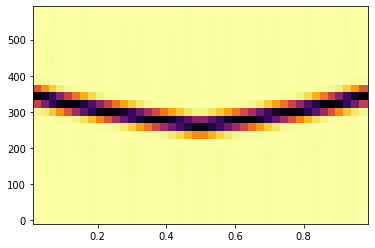
\includegraphics[width=0.75\textwidth]{ex5_spectrogram.png}
        \caption{Спектрограмма}
        \label{fig:ex5_spectrogram}
    \end{figure}
    
    На глаз она кажется кусочно-линейной, но из рассуждений выше следует, что это лишь иллюзия.
    
    \chapter{Гласные}
    
    Скачаем какие-нибудь звуки гласных из сети и посмотрим на них.
    
\begin{lstlisting}[language=Python,caption=Выбираем участок]
wave = read_wave(
    'Sounds/523055__cbelloso__vocales-vowels-man-woman-kid-girl.wav'
)
segment = wave.segment(start=0.2, duration=3.9)
segment.plot()
\end{lstlisting}

    \begin{figure}[H]
        \centering
        \includegraphics[width=0.75\textwidth]{ex6_spectrгm.png}
        \caption{Участок}
        \label{fig:ex6_spectrгm}
    \end{figure}
    
\begin{lstlisting}[language=Python,caption=Спектрограмма]
segment.make_spectrogram(512).plot()
\end{lstlisting}

    \begin{figure}[H]
        \centering
        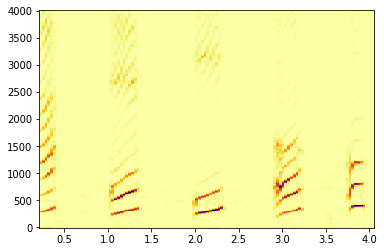
\includegraphics[width=0.75\textwidth]{ex6_spectrogram.png}
        \caption{Спектрограмма}
        \label{fig:ex6_spectrogram}
    \end{figure}
    
    Участки не горизонтальны потому, что так звуки произноятся на записи. Нам важно то, что некоторые из участков темнее, а некоторые светлее (в рамках одного столбца), что соответствует спектрам соответствующих гласных.
    
    В \texttt{.ipynb}-файле этой лабораторной работы можно посмотреть на сами спектры гласных. Я не стал вставлять их сюда, потому что это утомительно.
    
\end{document}
